\section{接受使用\TeX 撰写的毕业论文}[Advices on Acceptance for Dissertation Typesetting with \TeX]
\subsection{提议原因}[Reasoning]
\ppt{引入\TeX :开明之举}
在第\ref{sec:texBene}节中,我们讨论了在学术论文排版时使用\TeX 的优越性。\cquthesis 使得毕业生能够以很低的排版时间代价得到格式规范,排版质量高,索引目录齐全,美观大方的毕业论文。但是,\TeX 对于许多同学来说却是百分百的新事物(尽管\TeX 发行于1978年),学校官方的表态无疑会为许多对\TeX 有兴趣却烦恼没有用武之地的同学提供学习的动力。

\ppt{引入\TeX :民心所向}
当前,我校教务处以及研究生院对是否接受\TeX 撰写的毕业论文这一问题态度模糊。在我校民主湖论坛上,针对这一问题有很多讨论,以下是一些典型的帖子:
\begin{itemize}
	\item \href{http://www.cqumzh.cn/bbs/forum.php?mod=viewthread&tid=830829}{请投票支持论文采用\LaTeX 排版}
	\item \href{http://www.cqumzh.cn/bbs/forum.php?mod=viewthread&tid=830608}{[讨论] 重大的博士论文为什么木有\LaTeX 模版?}
	\item \href{http://www.cqumzh.cn/bbs/forum.php?mod=viewthread&tid=264031}{[理工科学] 有用\LaTeX 写论文的吗?交流一下 }
	\item \href{http://www.cqumzh.cn/bbs/forum.php?mod=viewthread&tid=931065}{博士毕业论文用\LaTeX 排版,之后的提交什么的会麻烦么?}
	\item \href{http://www.cqumzh.cn/bbs/forum.php?mod=viewthread&tid=936958}{重庆大学自己的毕业论文\LaTeX 模板来啦!}
	\item \href{http://www.cqumzh.cn/bbs/forum.php?mod=viewthread&tid=615852}{[编程] [求助]关于\LaTeX}
	\item \href{http://www.cqumzh.cn/bbs/forum.php?mod=viewthread&tid=818609}{被\LaTeX 所征服}
\end{itemize}

帖子的时间跨度从2006年至今,可以看出,至少在十年以来,我校师生中一直存在着\TeX 用户。在帖子中,他们的情感主要着力于以下几点:1. 认识到\TeX 很强大,主观上很想使用\TeX 进行毕业论文排版;2. 对教务处(本科生)或研究生院(研究生)是否接受使用\TeX 排版的论文心存顾虑,感到烦恼;3. (研究生)对研究生院毕业论文收费排版的现状\footnote{笔者对研究生院要求绝大多数研究生以1元/页的价格购买官方指定的排版服务的做法深表遗憾。}感到愤怒和无奈;4. 学习\TeX 遇到困难,感到求助无门。

在帖子\href{http://www.cqumzh.cn/bbs/forum.php?mod=viewthread&tid=830829}{请投票支持论文采用\LaTeX 排版}中,发帖人luoluo114\footnote{按照民主湖论坛的账号政策,民主湖论坛内的用户都是重庆大学学子。}发起了投票,他说道\footnote{原文引用,不改变错别字或错误用法,例如“latex”应该写为“LaTeX”,或者“\LaTeX ”,下同。}:

\begin{quotation}
	为避免我们的下一届学弟学妹身受格式痛苦,我觉得有必要发起该投票。latex其优点是有目共睹的,希望研院发起这样一个模板,或者承认latex格式的论文,让大家把精力应用于论文质量而不是格式本身。
	
	本人曾用word写毕业论文,因参考文献标号不是从1开始而花在修改编号上的时间用了一天。 而利用latex,仅仅是几分钟的事情。
\end{quotation}

在参与投票的246名重大学子中,有162名投票希望使用\LaTeX 排版,51名希望使用Word排版,33名没有表态,票数之间大小关系如\autoref{fig:tex-word-vote}所示。

\begin{figure}[tbh]
\centering
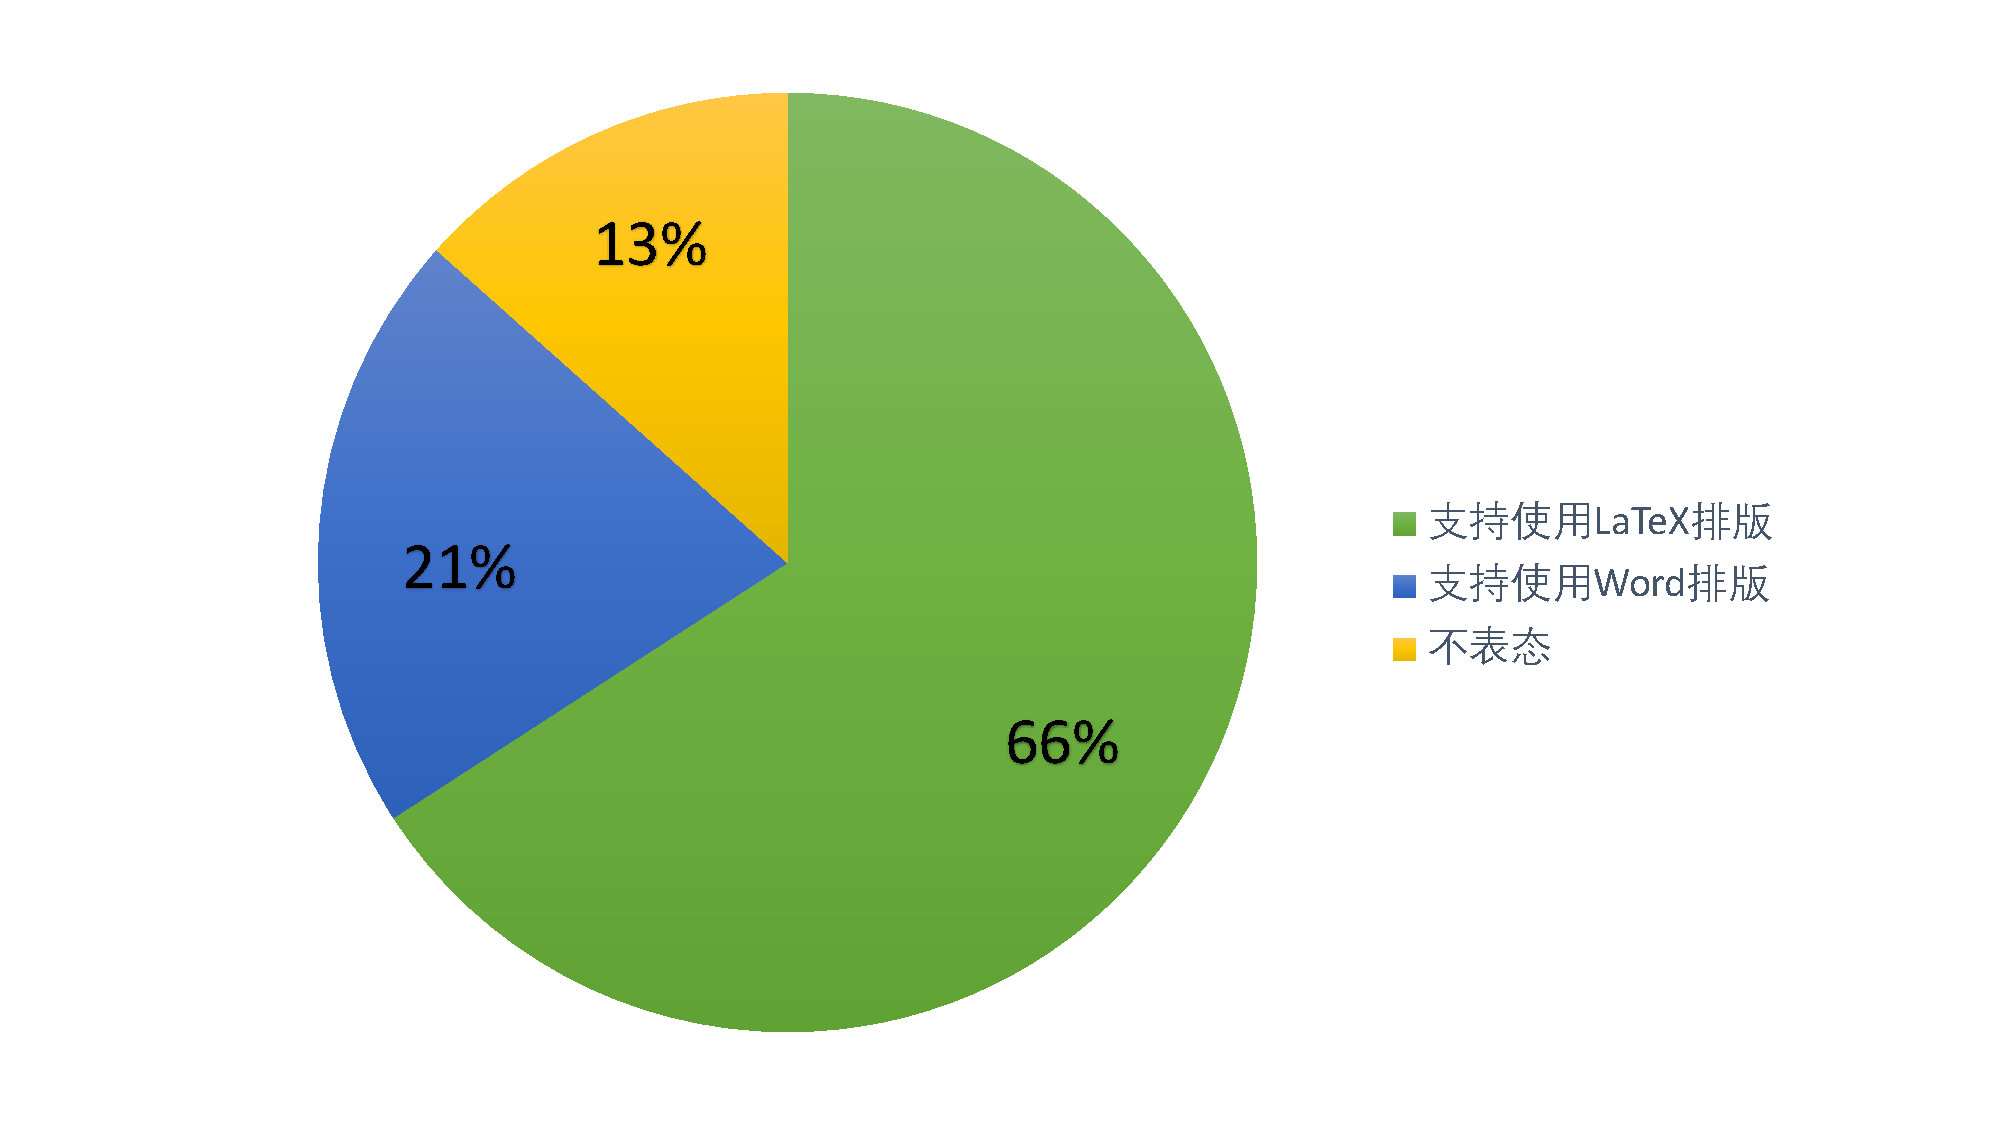
\includegraphics[width=\linewidth]{figures/TeX-Word-Vote}
\caption{民主湖中使用\LaTeX 进行毕业论文排版的支持率}
\label{fig:tex-word-vote}
\end{figure}

笔者另外节录了一些有思想性的观点,以飨读者:
\begin{quotation}
	这个建议官方做不是太靠谱,一般学校都是latex版面的爱好者自己做的 。
	很多学校都有自己的版本,上海交大,中国科大等,都是基于CASthesis 的。
	其实论文格式要求都差不多,拿过来修改下就可以了。
	用latex写论文,还是比较方便的,不太熟悉 tex的人照模块做基本都能做到。
	\par\hfill ——paulsum
	
	latex入手较慢,不过常用的功能很好掌握。
	熟练以后论文排版很快,而且整齐划一。
	\par\hfill ——cqustone
	
	Latex最重要的是排版规范,格式基本不会出错,如果学校能组织一帮同学做个模板,或者说承认同学的Latex排板,会给写论文带来极大方便。因为你关注是论文本身,而不会再去关注格式!这一点word是做不到的。
	
	word编号是没有问题,但我想大部分同学都遇到过文章长了之后格式不对的情况,什么编号缩进不对,前后文字体不对等等。而对于latex来说,你只需要知道此处应该有编号就可以了,缩进字体这些提供的模板自然会帮你处理。
	\par\hfill ——chengfzy
	
	这不是砸人家饭碗吗?你知道采用LATEX编辑,(研究生院指定的排版机构)要少挣多少钱不?
	\par\hfill ——sxkcqu
	
	最近在用这个软件写论文,感觉功能强大,但是又比较难学,经常为一个小问题卡壳,希望有同样爱好者交流一下!
	\par\hfill ——woodhead
	
	有没有什么地方必须提交word版的?用Latex排版然后提交生成的pdf可以么?有毕业了的师兄师姐是用的网上那个重大的Latex模板完成毕业论文的么?
	\par\hfill ——dashashi
	
	重大不让。如果可以的话省去很多麻烦。公式这些都不用去敲了。也不用去为格式操心,latex格式是固定的,不会出错。
	\par\hfill ——240536501
	
	前段时间了解了一些基础知识,现在意识到它的强大了。不在于能记忆多少,只要能很好的利用template完成自己的工作,那么Latex就为你节约了时间。这是它设计的目的之一。
	
	期待重大学位论文退出Latex的模板。
	\par\hfill ——八五折
	
	为设计者nanmu点赞!
	
	同时也希望研究生院相关部门大力支持,并推进其完善以至于形成正式版本,让更多的同学受益。
	
	Latex的广泛性和重要性不言而喻(基本覆盖了所有知名的国际期刊和出版集团,国内期刊也在大力推广),既然有专业人士用于尝试(如计者nanmu),相关部门更该顺势推进,成功推广必然对研究生学位论文相关工作起到巨大促进作用。而如果对此不予支持,甚至提出质疑,着实让人遗憾!
	
	试想这样一个场景,一位在国际知名期刊发表多篇高级别论文的博士生(小论文均为Latex版本),却要在答辩之前,花费大量时间精力用于研究latex与word之间的转化问题(笔者有过此经历,可谓“深受其害”),实在让人抓狂。希望这种情况不要再发生在各位在读的小伙伴身上了!
	\par\hfill ——supermtd
\end{quotation}

综合上述内容,学校联合教务处、研究生院表态接受使用\TeX 撰写的毕业论文是民心所向,也是引入先进工具先进思想的开明之举。

\subsection{依赖条件}[Dependencies]
\begin{enumerate}
	\item 论文存档方面,PDF文件本身的设计意图之一便是用于存档\cite{pdfISO},其格式稳定、规范\footnote{ISO 19005-3:2012},高度向后兼容,适合文件长期存档;
	\item 论文查重方面,大部分论文查重机构都能够对PDF文件格式的论文进行查重工作;
	\item 学校开设\TeX 培训课程(参阅第\ref{sec:texCourses}章);
	\item 学校完成CTAN镜像搭建(参阅第\ref{sec:ctanMirror}章)。
\end{enumerate}

\subsection{具体措施}[Detailed Measures]
措施可分为三步,表态、测试和推荐、维护。

\begin{enumerate}
	\item 表态:学校联合教务处、研究生院发文,表示接受使用\TeX 排版的PDF格式的论文,并确认提交PDF格式的论文和提交Word格式的论文完全等效,同时规定,无论论文的文件格式是什么,排版方式是什么,其格式以及书写规范都要符合重庆大学《重庆大学本科设计(论文)撰写规范化要求(2007年修订版)》和《重庆大学博士、硕士论文撰写格式标准(2007年修订版)》的要求;
	\item 测试和推荐:学校组织格式审查委员会对\cquthesis 的排版情况进行审查,确认其排版合规的情况下,在教务处和研究生院的毕业论文系统中添加\cquthesis 的说明介绍、用户文档和下载地址,起到对\TeX 用户的指导效果;
	\item 维护:学校保持对CTAN镜像的维护(参阅第\ref{sec:ctanMirror}章),并且保持对\TeX 培训课程(请参阅第\ref{sec:texCourses}章)的支持,如此这般,重庆大学师生的学术写作水平会在一定程度上得到长足提升,并且生生不息。
\end{enumerate}

\cquthesis 的技术维护由\href{https://github.com/nanmu42/}{李振楠}和\href{http://jq.qq.com/?_wv=1027&k=2HvYu95}{重庆大学\TeX 用户组}进行。